\section{Problemstilling}
Reinseanlegget er teknisk utdatert og er avhengig av modernisering. Stryringssystemet er over tjue år gammalt
og består hovudsakeleg av eldre og utgåtte komponentar. Med eldre komponentar aukar risikoen for svikt, 
og reservedelar som passar kan være vanskeleg å finne.

WaterCare, som leverte styresystemet er i seinare tid også blitt avvikla noko som gjer at kompetansen 
og moglegheiten for å gjere endringar i styresystemet er vankeleg. 
Mykje grunna denne utfordrina har ikkje anlegget følgt den teknologiske framdrifta 
og små problem har samla seg opp til å bli større utfordringar.

Samtidig med desse faktorane er dokumentasjonen til reiseanlegget dårleg noko som gjer at enkle arbeidsoppgåver blir lange og tunge.
I eit værste tilfelle vil styringseinheten på anlegget svikte og med det som er nevnt tidlegare vil det være krevjande
å få anlegget i drift igjen. Dette er eit kritisk problem innan avlaupshandtering og kan ikkje sjåast vekk ifrå.
\newline

%\begin{figure}[htbp]
%    \centering
%    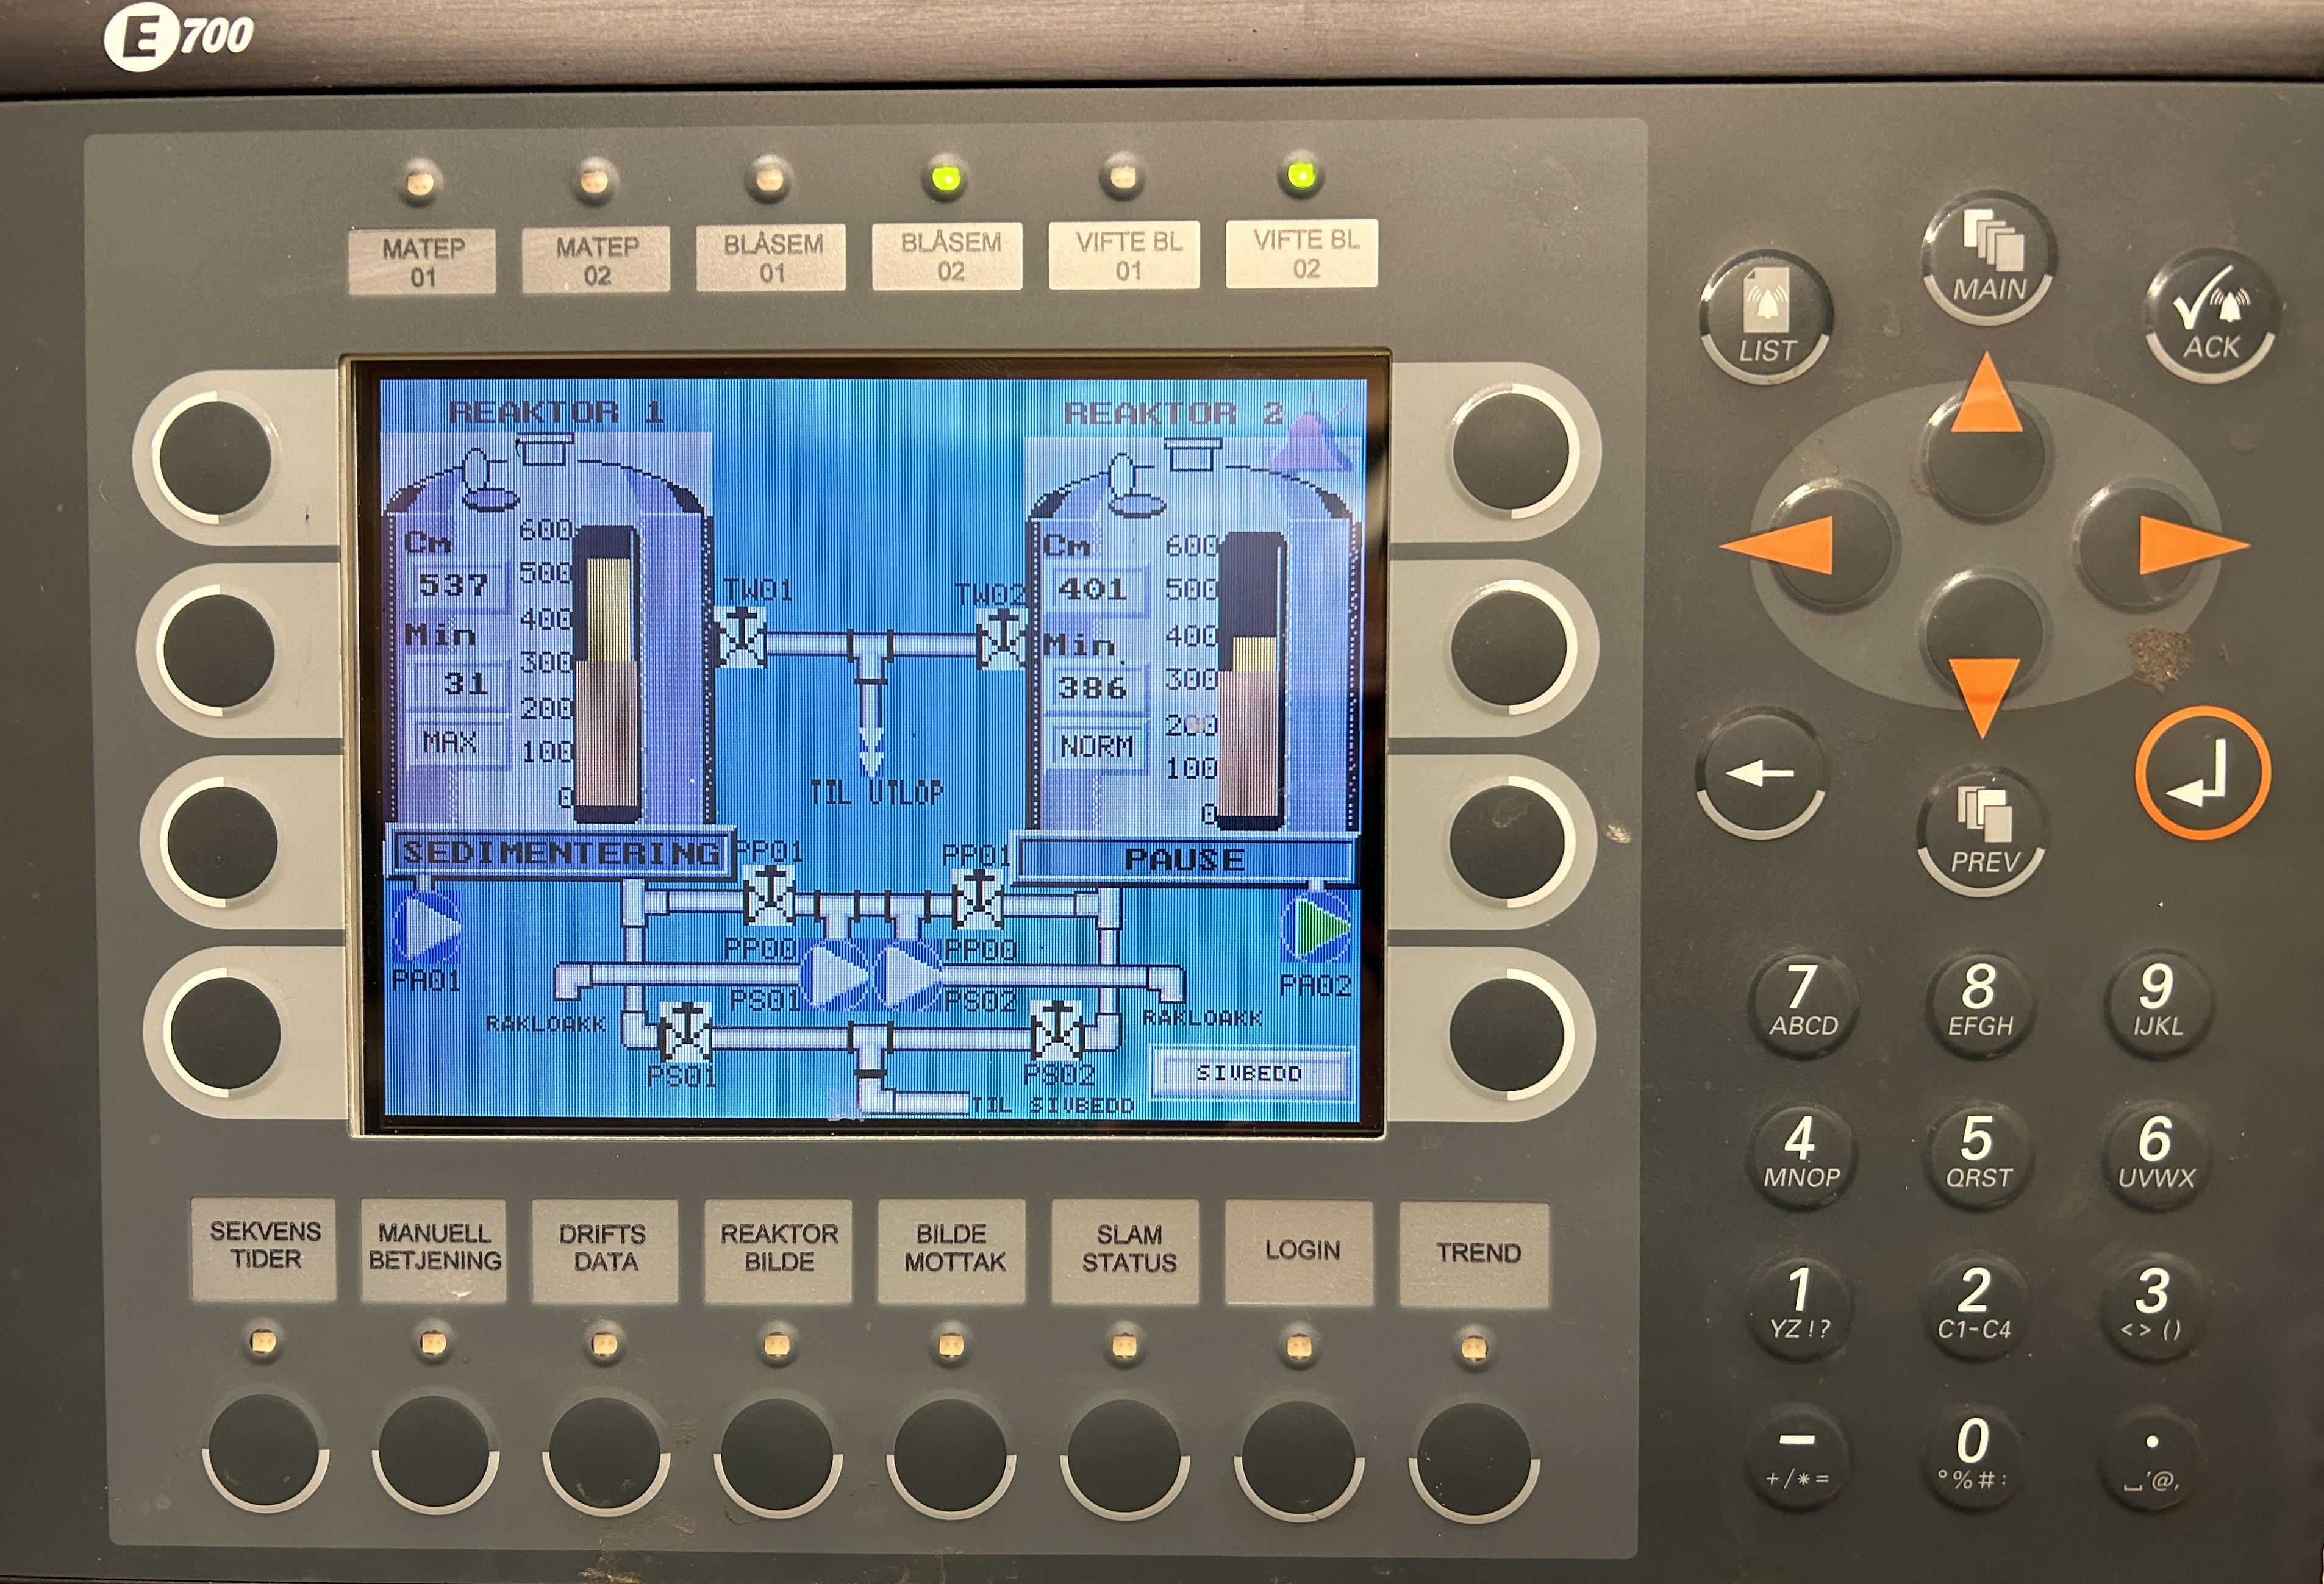
\includegraphics[width=0.8\textwidth]{Bilder/BeijerSkjerm.JPG}
%    \caption{Beijer HMI}\label{fig:HMI}
%\end{figure}


\begin{figure}[htbp]
    \centering
    \begin{subfigure}[b]{0.5\textwidth}
        \centering
        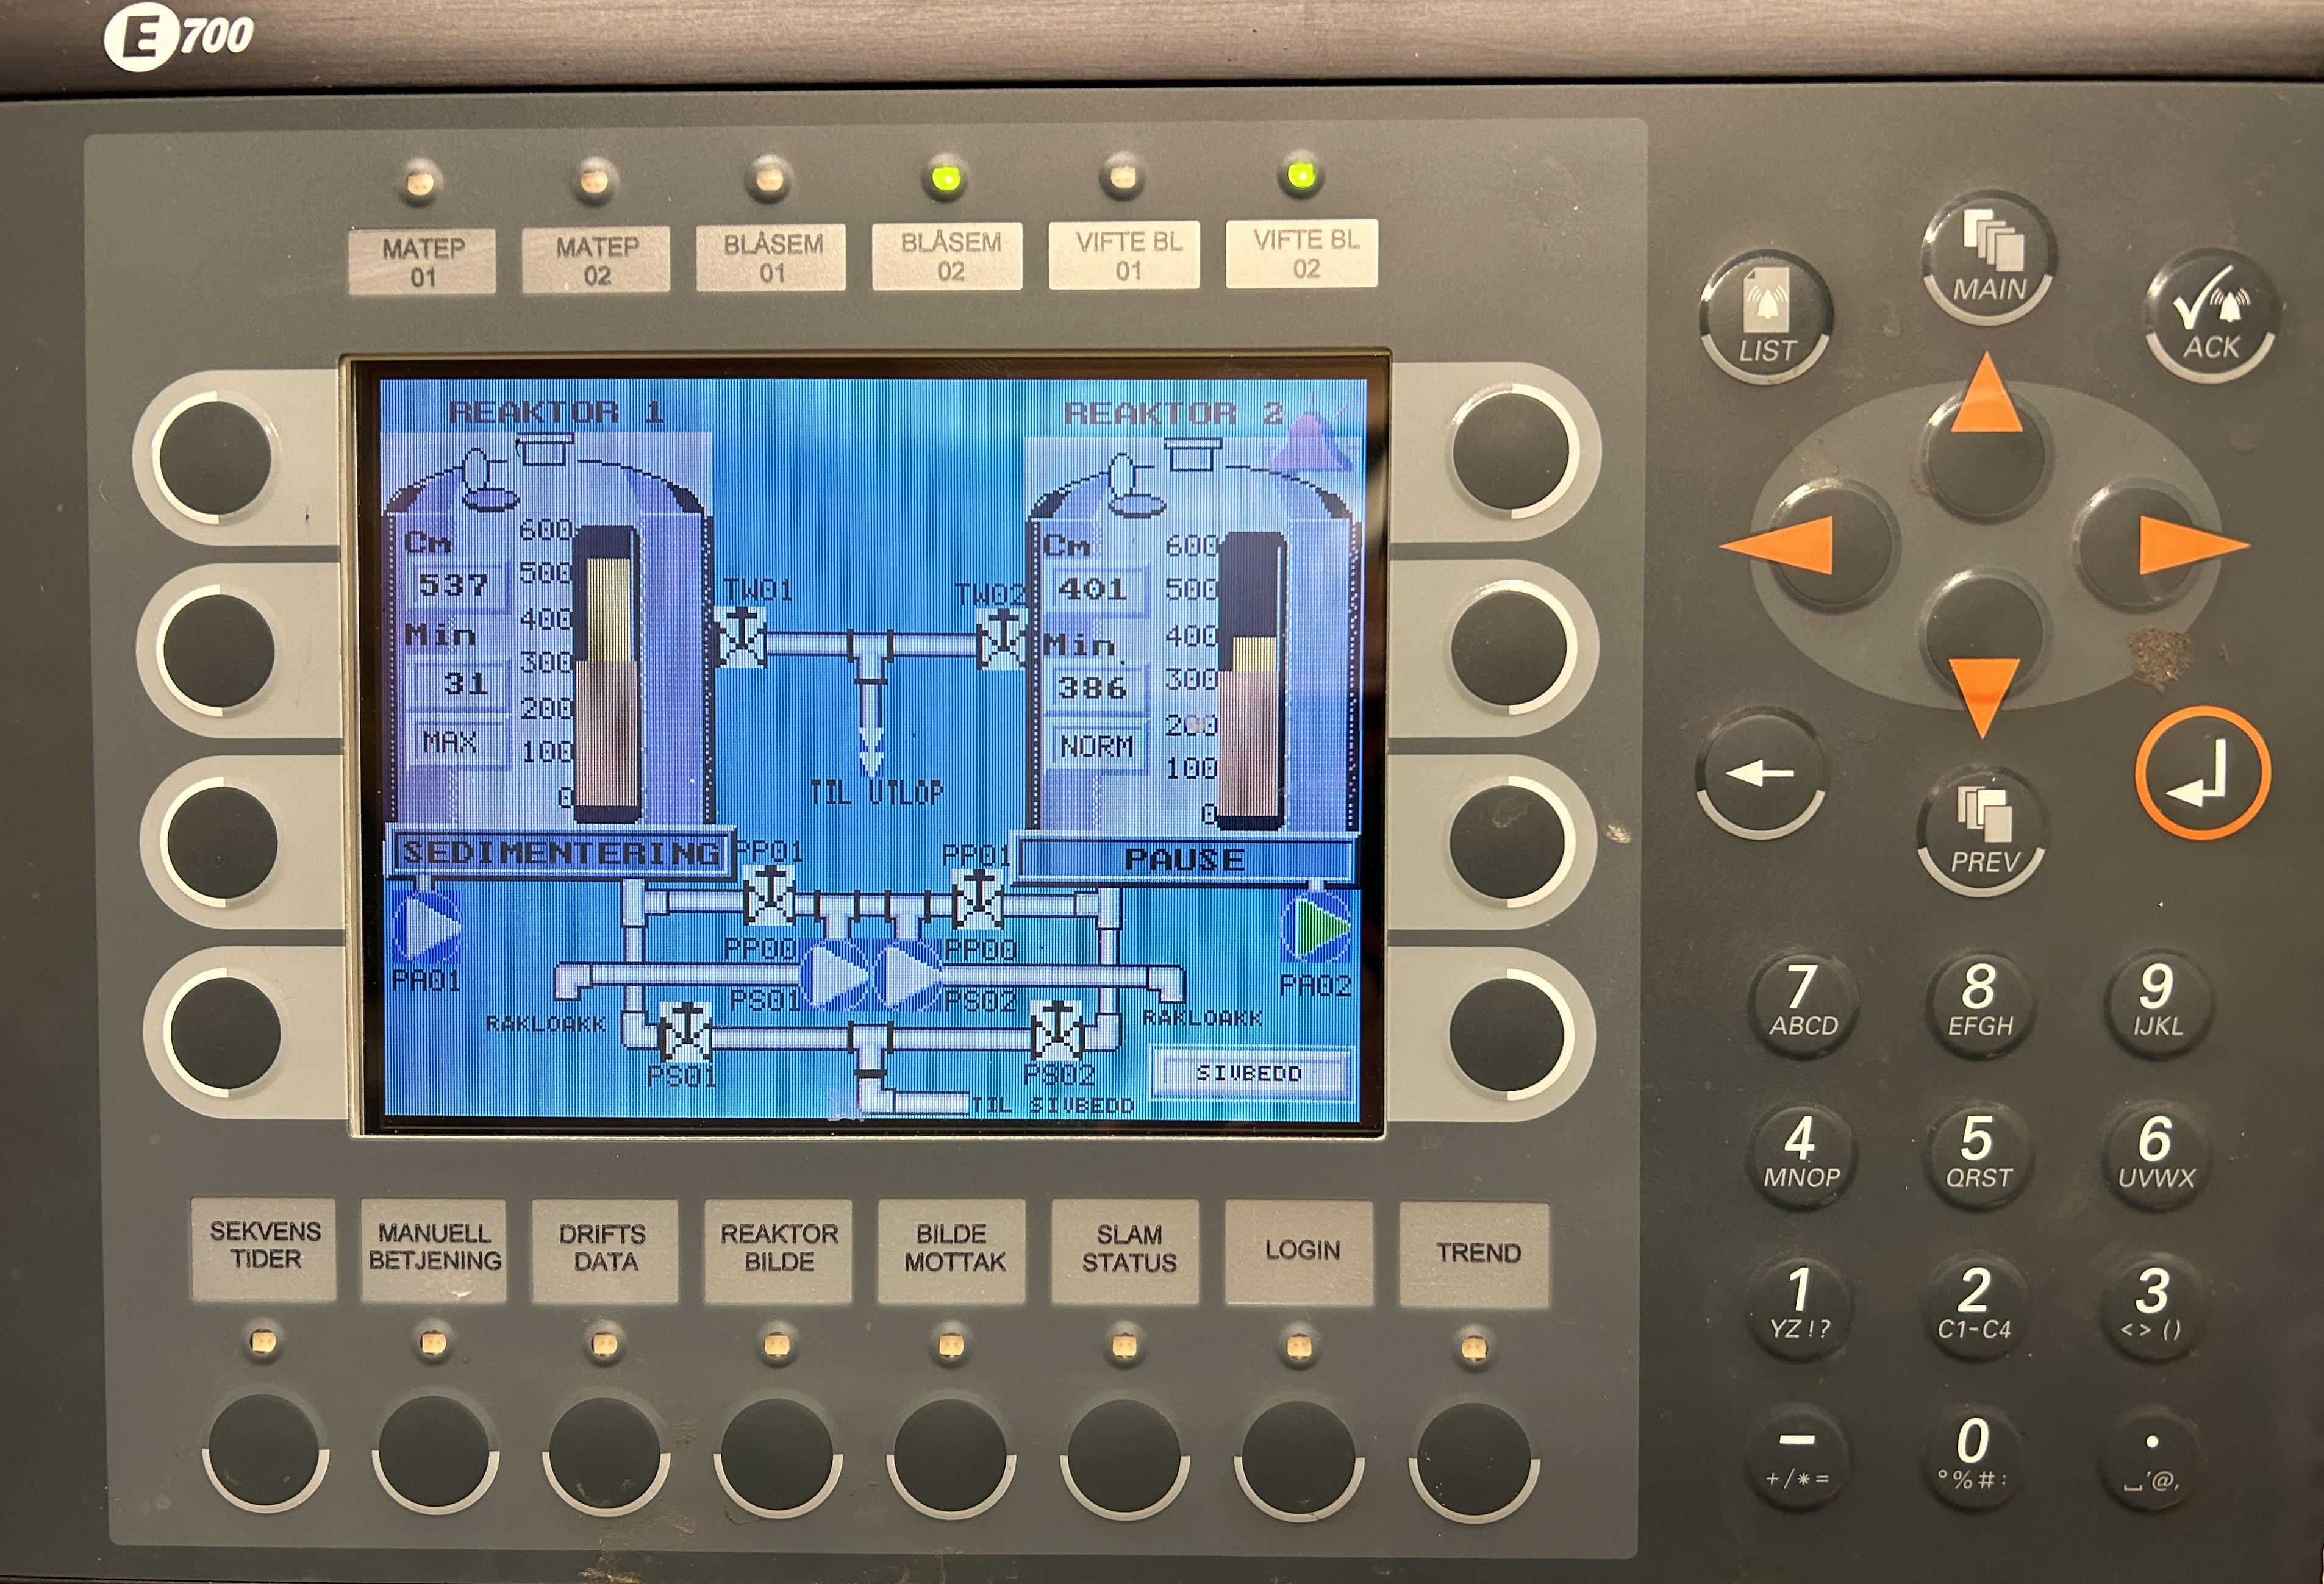
\includegraphics[width=1\textwidth]{Bilder/BeijerSkjerm.JPG}
        \caption{Beijer HMI}\label{fig:subfig1}
    \end{subfigure}
    \hfill
    \begin{subfigure}[b]{0.3\textwidth}
        \centering
        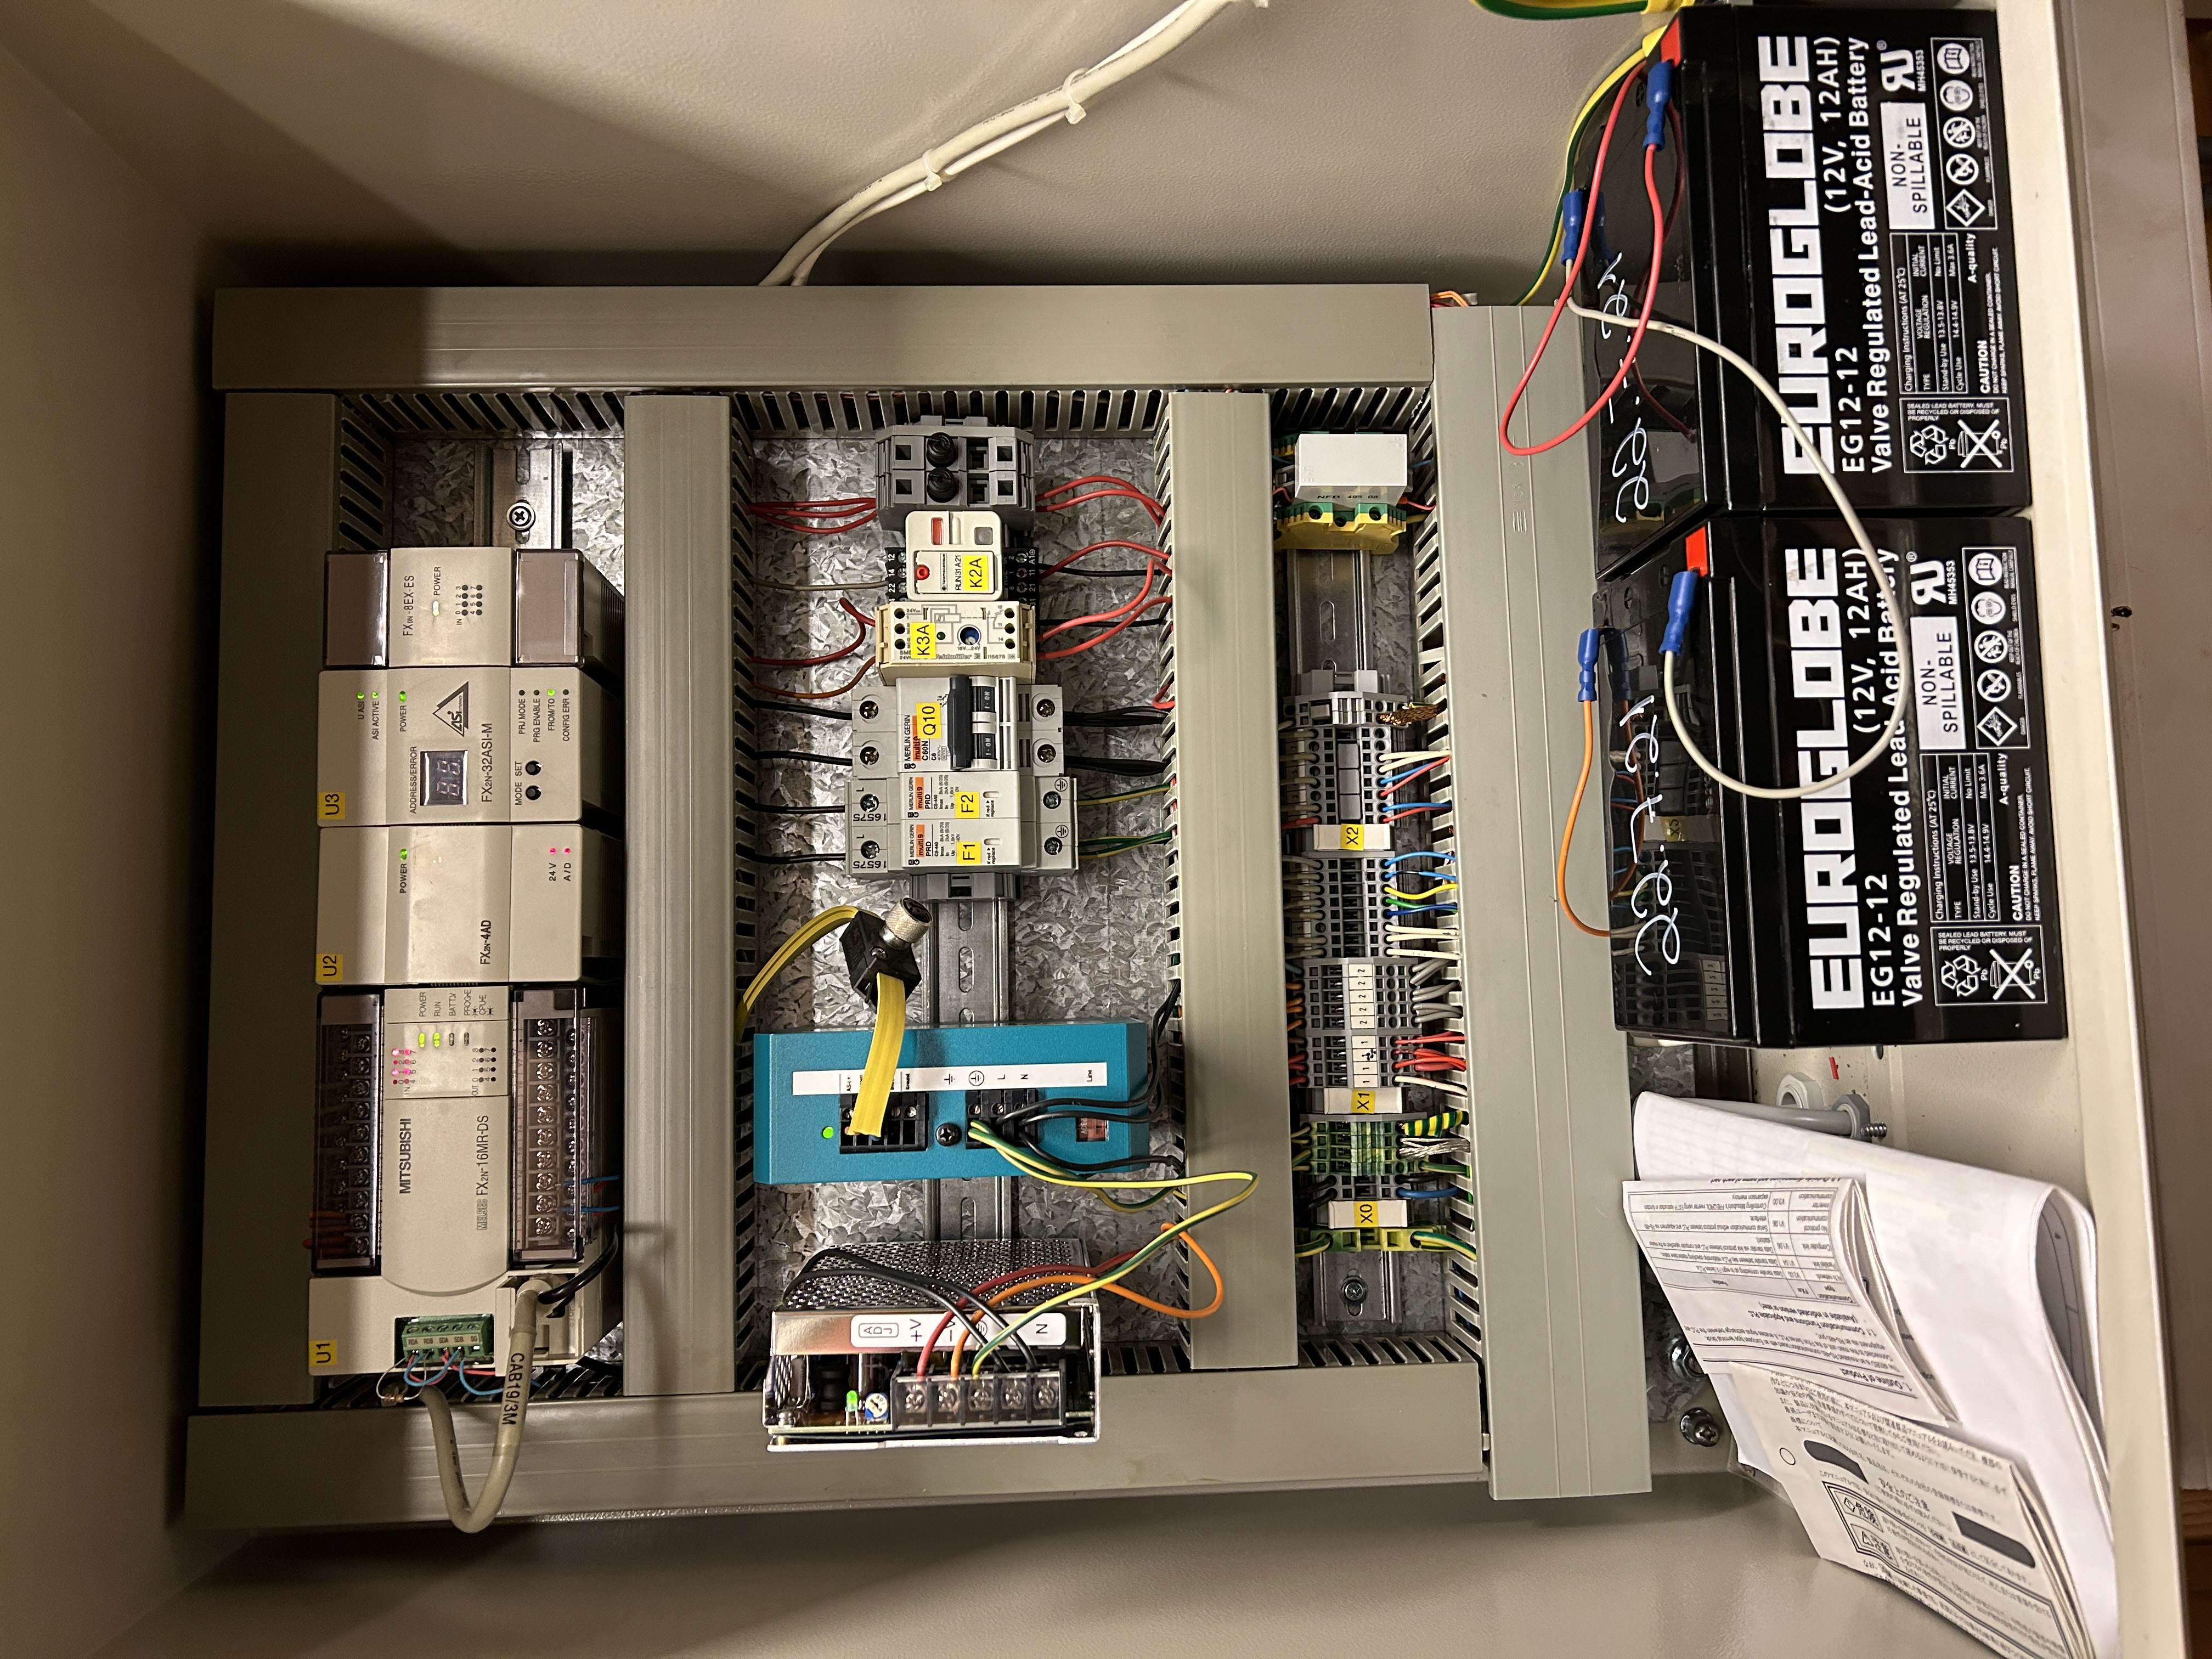
\includegraphics[angle=-90,width=1\textwidth]{Bilder/Styreskap.JPG}
        \caption{Styreskap}\label{fig:subfig2}
    \end{subfigure}
    \caption{Styresystem}\label{fig:Styresystem}
\end{figure}